\section{Preprocessing}
\setcounter{figure}{0}
\renewcommand{\thefigure}{4.\arabic{figure}}\\
\quad In this chapter, we will explore the preprocessing stage of our Braille
Translator system. We chose to implement a step-by-step approach,
gradually increasing complexity, rather than using all the filters from
the beginning. First, we will describe the challenges we encountered and
the phases we went through before discussing the filters used to address
these issues.

\hypertarget{development-phases}{%
\subsection{Development Phases}\label{development-phases}}\\
\quad Scanned papers often present various challenges, such as scanner noise, paper skewing, and damage due to being held too tightly. To address these issues effectively, we decided to begin our work with low complexity and gradually increase it, experimenting with different sources of noise at each step.\\
\hypertarget{Sample input 0}{%
\subsubsection{Sample input 0}\label{Sample input 0}}\\
\quad Recognizing the complexity of image processing tasks, we decided to
start with a flawless input initially. This approach
allowed us to test the functionality of our system before introducing
real-world application challenges.

\begin{figure}[h!]
     \centering
     \begin{subfigure}
         \centering
         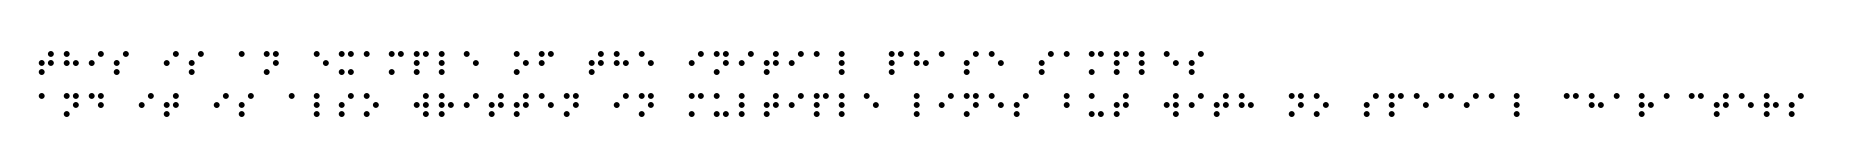
\includegraphics[width=\textwidth]{image1.png}
         \label{fig:Perfect braille image}
     \end{subfigure}
     \begin{subfigure}
         \centering
         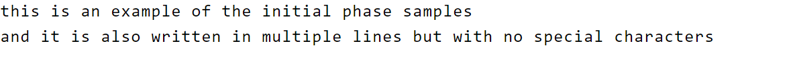
\includegraphics[width=\textwidth]{image2.png}
         \label{fig:Corresponding text}
     \end{subfigure}
        \caption{Braille writing using software tool}
        \label{fig:Braille writing using software tool}
\end{figure}\\
\quad We utilized a free online software tool that converts text to Braille characters, producing images with perfect dot sizing and coloring, and
free from noise, corruption, and rotation.\\

\hypertarget{Sample input 1}{%
\subsubsection{Sample input 1}\label{Sample input 1}}
\vspace{1em}\\
\quad During this phase, we faced one of the most significant challenges of
our project: Braille printing. Braille printers are rare, and although
we found a few, we could only gain limited access to one of them.\\

\quad We printed two pages with perfect specifications, free of noise and
errors. During this phase, we encountered some challenges and needed to
determine the optimal scanning method and quality to achieve the best
accuracy within a reasonable timeframe. We scanned the pages at 100 DPI,
concluding that this was a critical configuration point.\\

\quad In this phase, we sidestepped translation issues and treated the
program as separate modules. This approach allowed us to manage each
component individually before merging them back into the main program
branch in our workflow.\\
\clearpage
\begin{figure}[h!]
     \centering
         \centering
         
\includegraphics[width=.8\textwidth]{image5.jpg}
        \caption{Clear real braille samples}
        \label{fig:Clear real braille samples}
\end{figure}\\

\quad The primary challenge was to convert the scanned image into the clearest
possible version, like the ideal image used in phase 0. The filter stage
played a crucial role in this process. By applying specific filters such as Otsu's thresholding, GaussianBlur and medianBlur, we were able to enhance the clarity of the scanned image. These techniques will be discussed in detail later in this chapter.\\
\newpage
\hypertarget{Sample input 2}{%
\subsubsection{Sample input 2}\label{Sample input 2}}\\

\quad During this phase, we intentionally introduced various types of noise,
including light irregularities, corrupted pages, low-content pages, and
rotated pages. We successfully identified and categorized these issues,
resolving some while identifying others as critical points to avoid in
future processes.\\

\quad We will highlight the following critical points which we deem the
responsibility of the user:\\

\begin{enumerate}
\def\labelenumi{\arabic{enumi}.}
\item
  Users should refrain from gripping the paper too tightly to avoid
  damaging or distorting the dots.
\item
  Papers should be kept clean.
\item
  The scanner cover should be securely closed.
\end{enumerate}\\
\begin{figure}[h!]
    \centering
    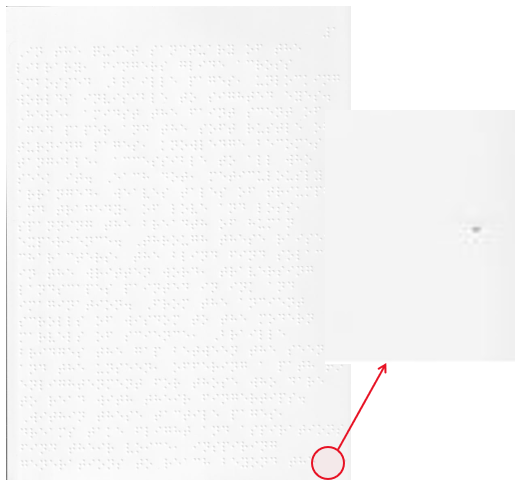
\includegraphics[width=.9\textwidth,height = 10cm]{A drop of dirt.png}
    \caption{A drop of dirt causes system failure}
    \label{fig:Clear real braille samples}
\end{figure}
\begin{figure}
    \centering
    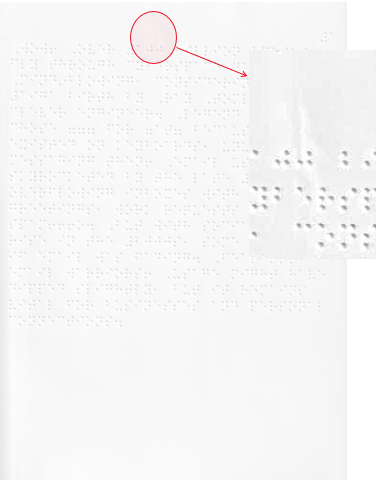
\includegraphics[width=.8\textwidth,height = 10cm]{held tight.png}
    \caption{Corrupted paper due to being held tight}
    \label{fig:Clear real braille samples}
\end{figure}\\
\begin{figure}[h!]
    \centering
    
\includegraphics[width=.9\textwidth,height = 10cm]{Low content.png}
    \caption{Low content pages contain light distribution irregularity}
    \label{fig:Clear real braille samples}
\end{figure}
\clearpage
\hypertarget{filters-and-opencv-methods-used}{%
\subsection{Filters and OpenCV methods
used}\label{filters-and-opencv-methods-used}}
\\
\quad Here is a block diagram illustrating the steps involved in our preprocessing system, which will be discussed in detail.\\
\begin{figure}[h!]
    \centering
    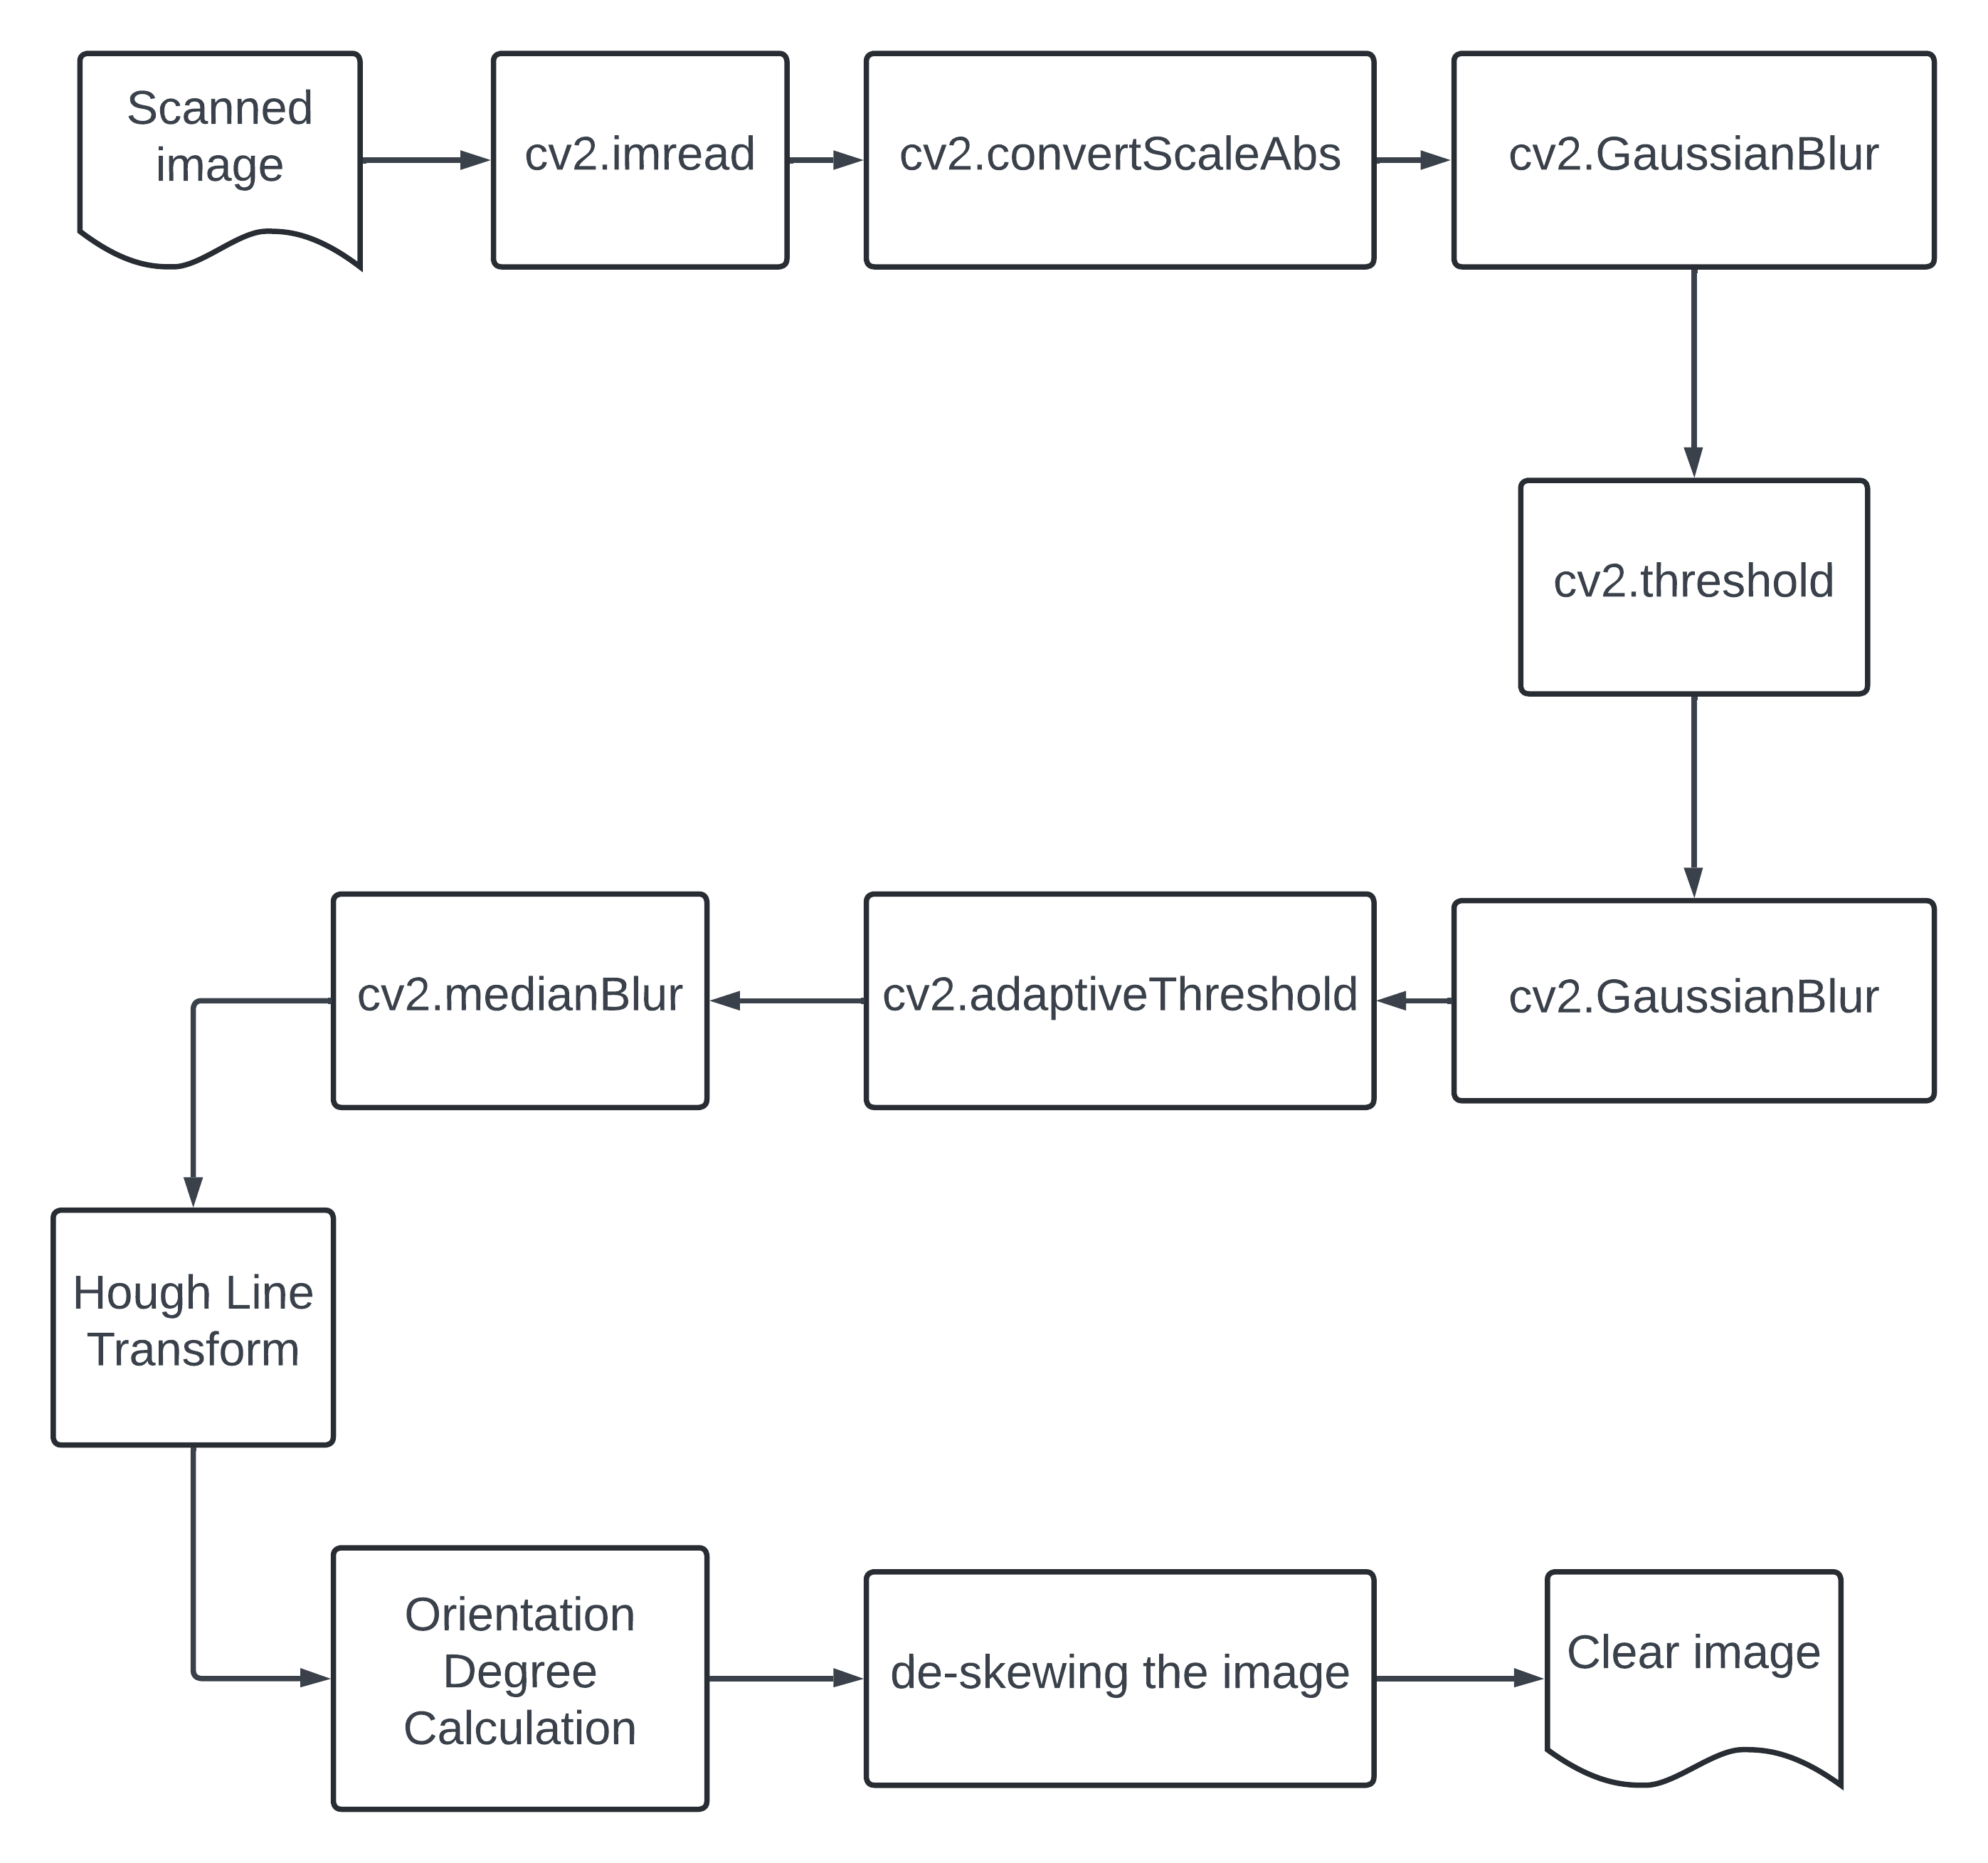
\includegraphics[width=.9\textwidth]{Preprocessing diagram.png}
    \caption{Preprocessing steps Diagram}
    \label{fig:Clear real braille samples}
\end{figure}
\newpage
\hypertarget{cv2.imread}{%
\subsubsection{cv2.imread}\label{cv2.imread}}

\begin{quote}
The method imread loads an image from the specified file and returns it.
\end{quote}\\

\begin{itemize}
\item
  The function determines the type of an image by the content, not by
  the file extension.
\item
  In the case of color images, the decoded images will have the channels
  stored in~\textbf{BGR}~order.
\item
  When using IMREAD\_GRAYSCALE, the codec\textquotesingle s internal
  grayscale conversion will be used, if available.
\item
  The dimensions of the scanned image using the scanner mentioned in the
  configuration section are (850 x 1169) at 100 DPI.
\end{itemize}\\


\begin{figure}[h!]
     \centering
        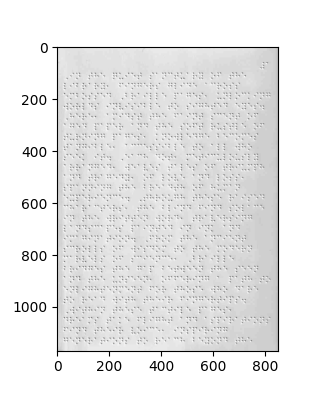
\includegraphics[width=0.8\textwidth,height=12cm]{image9.png}
        \caption{Scanned braille-written paper in general case}
        \label{fig:Scanned braille-written paper in general case}
\end{figure}\\


\hypertarget{cv2.convertscaleabs}{%
\subsubsection{cv2.convertScaleAbs}\label{cv2.convertscaleabs}}

\quad Scales, calculates absolute values, and converts the result to 8-bit.\\

\quad On each element of the input array, the function convertScaleAbs
performs three operations sequentially: scaling, taking an absolute
value, conversion to an unsigned 8-bit type:\\

\[dst(I) = saturate\backslash\text{\_}cast < uchar > (\left| src(I)*alpha + beta \right|)\]\\
\begin{itemize}
    \item \(\text{dst}(I)\): The destination pixel value at location \( I \).
    \item \(\text{src}(I)\): The source pixel value at location \( I \).
    \item \(\alpha\): A scaling factor applied to the source pixel values.
    \item \(\beta\): An added offset (brightness adjustment).
    \item \(\text{saturate\_cast}<\text{uchar}>\): Ensures the resulting value is clipped to the 8-bit range (0 to 255) and converted to an unsigned 8-bit type.
    \item \(| \ldots |\): Takes the absolute value of the expression inside.
\end{itemize}\\

\quad There are two tunable parameters which are alpha and beta, these
parameters have a huge impact in some special cases just as rotated
images and low content images.\\

\quad After a dedicated tuning session for these parameters to optimize the
mentioned special cases while maintaining the functionality in the
normal cases, it was proven that in our application alpha should be set
to (1.085) while beta performed just as required at a value of (-12).\\

\begin{figure}[h!]
     \centering
     \begin{subfigure}
         \centering
         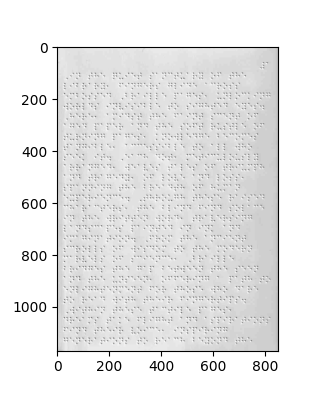
\includegraphics[width=.48\textwidth,height=8cm]{image9.png}
     \end{subfigure}
     \hfill
     \begin{subfigure}
         \centering
         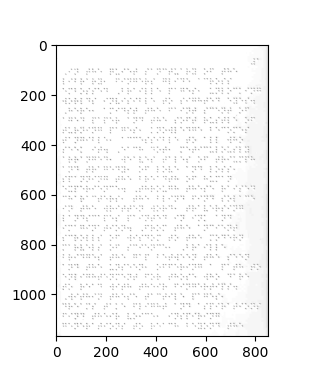
\includegraphics[width=.48\textwidth,height=8cm]{image11.png}
     \end{subfigure}
        \caption{Before and After applying convertscaleabs filter}
        \label{fig:Clear real braille samples}
\end{figure}\\

\newpage
\hypertarget{cv2.gaussianblur}{%
\subsubsection{cv2.GaussianBlur}\label{cv2.gaussianblur}}

Blurs an image using a Gaussian filter.\\

\quad The function convolves the source image with the specified Gaussian
kernel. In-place filtering is supported.\\

\quad We applied GaussianBlur twice due to its significant effect on noise
reduction. However, it must be used carefully to avoid erasing any
important data from the image. Here are some key functions of the
GaussianBlur filter in our application:\\

\begin{itemize}
\item
  \textbf{Noise Reduction}: The GaussianBlur filter effectively reduces
  noise by averaging the pixel values in a neighborhood defined by a
  Gaussian function. This helps in smoothing the image while preserving
  important structural details, making it easier to detect and recognize
  text or Braille dots.
\item
  \textbf{Edge Preservation}: Unlike other blurring techniques, the
  GaussianBlur filter maintains the integrity of edges, ensuring that
  the critical boundaries of characters or dots remain distinguishable.
  This is crucial for accurate feature extraction in subsequent
  processing stages.
\item
  \textbf{Preparation for Binarization}: GaussianBlur helps in creating
  a more uniform background, which is essential for effective
  binarization. A well-blurred image with uniform intensity levels
  facilitates better thresholding, resulting in a clearer distinction
  between the text/Braille dots and the background.
\item
  \textbf{Reducing Artifacts}: In images with varying light conditions,
  the GaussianBlur filter helps in reducing artifacts caused by shadows
  or uneven lighting. This normalization is important for maintaining
  consistency across different samples, ensuring reliable and repeatable
  results in the Braille translation process.
\end{itemize}\\
\begin{figure}[h!]
     \centering
     \begin{subfigure}
         \centering
         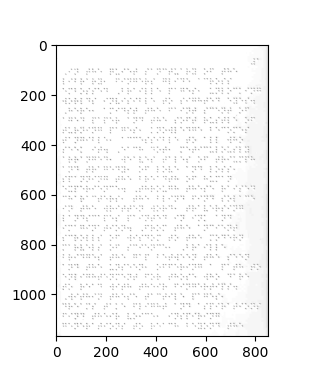
\includegraphics[width=.48\textwidth,height=8cm]{image11.png}
     \end{subfigure}
     \hfill
     \begin{subfigure}
         \centering
         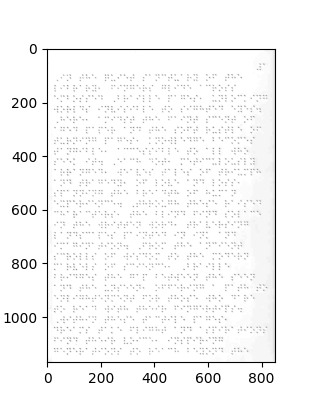
\includegraphics[width=.48\textwidth,height=8cm]{image13.png}
     \end{subfigure}
        \caption{Before and After applying the GaussianBlur filter}
        \label{fig:Clear real braille samples}
\end{figure}\\
\begin{quote}
Let's introduce the effect of the GaussianBlur filter on the previous image:
\end{quote}\\

\quad As shown in figure 4.7, GaussianBlur has a gentle effect on the edge
artifacts. It\textquotesingle s important to note
that at this stage, we used a mild GaussianBlur with a kernel of size 1
and a standard deviation of (1,1). These parameters will be adjusted
later to achieve a stronger blurring effect.\\
\newpage
\hypertarget{cv2.threshold}{%
\subsubsection{cv2.threshold}\label{cv2.threshold}}

\quad Applies a fixed-level threshold to each array element.\\

\quad The function applies fixed-level thresholding to a multiple-channel
array. The function is typically used to get a bi-level (binary) image
out of a grayscale image (compare~could be also used for this purpose)
or for removing a noise, that is, filtering out pixels with too small or
too large values. There are several types of thresholding supported by
the function. They are determined by type parameter.\\

\quad The special
values \textbf{THRESH\_OTSU} or \textbf{THRESH\_TRIANGLE}
be combined with one of various types of thresholding such as THRESH\_BIN and\\ THRESH\_BIN\_INV. In these cases, the function
determines the optimal threshold value using the Otsu\textquotesingle s
or Triangle algorithm and uses it instead of the specified threshold.\\

\quad \textbf{THRESH\_OTSU} is utilized in our application combined with\\ 
\textbf{THRESH\_BINARY} to simplify the task of converting the image
into a perfect black-and-white format. The significance of
Otsu\textquotesingle s thresholding lies in its ability to automatically
determine the optimal threshold value, enhancing the accuracy of the
binarization process. This method minimizes the variance within each
class of pixels, ensuring that the text stands out clearly against the
background, which is crucial for effective Braille translation. By using
Otsu\textquotesingle s thresholding, we enhance the reliability of our
preprocessing stage, making it easier to handle various image qualities
and conditions.\\

\quad This filter has 2 tunable parameters which are thresh (threshold value)
and maxval (maximum value to use with \textbf{THRESH\_BINARY} and \\
\textbf{THRESH\_BINARY\_INV} thresholding types)\\

\quad At this stage, we will obtain a clear image with low noise and high
contrast. We will reapply the GaussianBlur filter to further smooth the
image, maximizing the effectiveness of this step. This time, we will use
a stronger GaussianBlur with a variance of (3,3), as previously
mentioned. The results of each step in this stage are illustrated in the
following figures:  \\

\begin{figure}[h!]
     \centering
     \begin{subfigure}
         \centering
         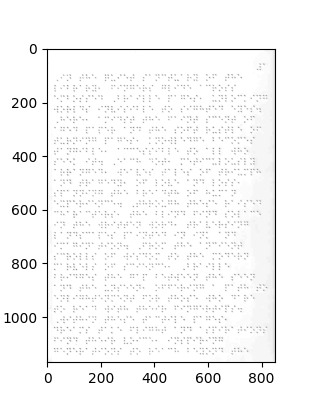
\includegraphics[width=.48\textwidth,height=8cm]{image13.png}
     \end{subfigure}
     \begin{subfigure}
         \centering
         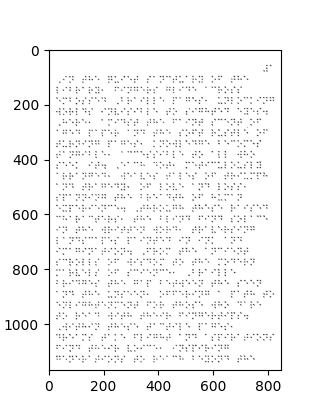
\includegraphics[width=.48\textwidth,height=8cm]{image15.png}
     \end{subfigure}
    \caption{Before and After Otsu's Threshold}
    \begin{subfigure}
    \centering
    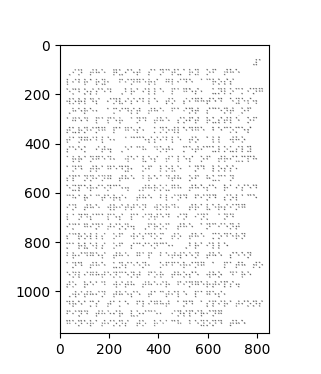
\includegraphics[width=.5\textwidth,height=8cm]{image16.png}
    \caption{After reapplying GaussianBlur}
    \label{fig:}
    \end{subfigure}
\end{figure}
\newpage
\hypertarget{cv2.adaptivethreshold}{%
\subsubsection{cv2.adaptiveThreshold}\label{cv2.adaptivethreshold}}\\

\quad In the previous section, we used a global value as threshold value. But
it may not be good in all the conditions where image has different
lighting conditions in different areas. In that case, we go for adaptive
thresholding. In this, the algorithm calculate the threshold for a small
regions of the image. So we get different thresholds for different
regions of the same image and it gives us better results for images with
varying illumination. So we can get the best case through this stage.\\

\quad The challenging aspect of this filter lies in fine-tuning its parameters
in conjunction with the previous stages to harness the benefits of
adaptive thresholding while avoiding its potential drawbacks in case of
inaccurate tuning. The key parameters are:\\

\begin{itemize}
\item
  \textbf{maxValue}: The non-zero value assigned to pixels that meet the
  condition.
\item
  \textbf{blockSize}: The size of the pixel neighborhood used to
  calculate the threshold value, typically an odd number like 3, 5, 7,
  and so on.
\item
  \textbf{C}: A constant subtracted from the mean or weighted mean,
  which can be positive, zero, or negative.
\end{itemize}\\

\quad For our purposes, these parameters were set to:\\

\begin{itemize}
\item
  \textbf{maxValue}: 255, since the background is pure white.
\item
  \textbf{blockSize}: 9
\item
  \textbf{C}: 21
\end{itemize}\\

\quad These values were determined through a trial-and-error tuning session.\\

\quad We can recognize from fig.4.12 that in this stage we have almost the
perfect image with high contrast, low noise which could be enough for
most cases but for some low content pages this stage is not enough so we
will go through the last and final filter in the next stage.\\

\begin{figure}[h!]
     \centering
     \begin{subfigure}
         \centering
         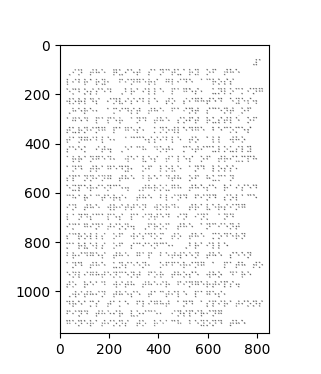
\includegraphics[width=.49\textwidth,height=8cm]{image16.png}
     \end{subfigure}
     \hfill
     \begin{subfigure}
         \centering
         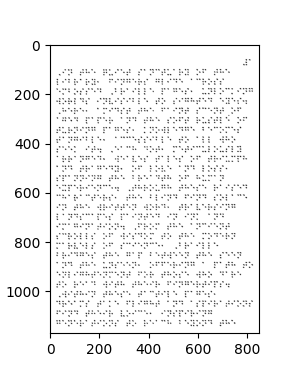
\includegraphics[width=.47\textwidth,height=8cm]{image19.png}
     \end{subfigure}
        \caption{Before and After applying AdaptiveThreshold}
        \label{fig:Clear real braille samples}
\end{figure}\\
\newpage
\hypertarget{cv2.medianblur}{%
\subsubsection{cv2.medianBlur}\label{cv2.medianBlur}}\\

\quad Median Blur is a powerful image processing filter that offers several
benefits, particularly in the context of noise reduction and edge
preservation:\\

\begin{itemize}
\item
  \textbf{Noise Reduction}: Median Blur is highly effective at reducing
  \textquotesingle salt-and-pepper\textquotesingle{} noise, a type of
  noise characterized by random bright and dark pixels scattered
  throughout the image.
\item
  \textbf{Edge Preservation}: Unlike other blurring techniques, Median
  Blur preserves edges while smoothing the image. which doesn\textquotesingle t blur sharp
  edges.
\item
  \textbf{Detail Retention}: It maintains the finer details in the
  image, making it useful for preprocessing steps where preserving
  important features is crucial.
\end{itemize}\\

\quad While Median Blur offers significant benefits, it also comes with
challenges:\\

\begin{itemize}
\item
  \textbf{Computational Intensity}: Median Blur can be computationally
  intensive, especially for large images or high kernel sizes, as it
  requires sorting the pixel values within the kernel for each pixel.
\item
  \textbf{Parameter Tuning}: Finding the optimal kernel size is critical
  and can be challenging. An inappropriate kernel size may either fail
  to remove noise effectively or excessively smooth the image, losing
  important details.
\end{itemize}\\

\begin{quote}
\quad The previous points show that the most important point to get the most
out of this filter is to perfectly identify the kernel size, the best
method to tune it is by starting with a small kernel and gradually
increase it to get the best accuracy with lowest computational power.\\

\begin{figure}[h!]
     \centering
     \begin{subfigure}
         \centering
         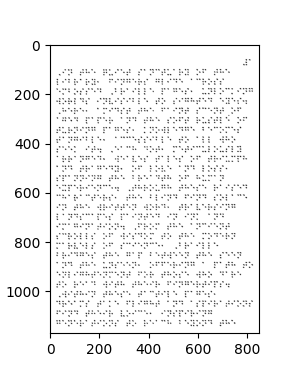
\includegraphics[width=.48\textwidth,height=8cm]{image19.png}
     \end{subfigure}
     \hfill
     \begin{subfigure}
         \centering
         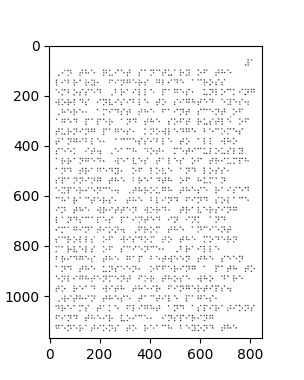
\includegraphics[width=.48\textwidth,height=8cm]{image21.png}
     \end{subfigure}
        \caption{Before and After applying the MedianBlur}
        \label{fig:Clear real braille samples}
\end{figure}
\newpage
\begin{figure}[h!]
     \centering
     \begin{subfigure}
         \centering
         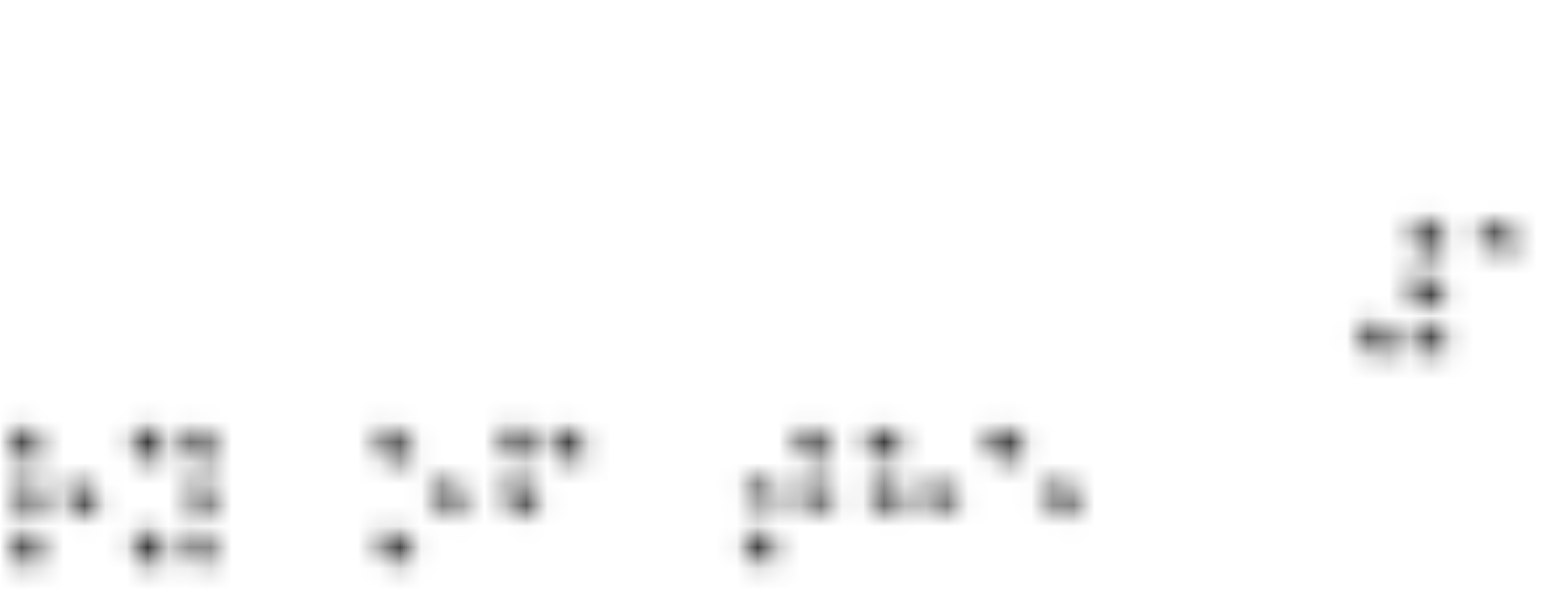
\includegraphics[width=.8\textwidth]{Before medianBlur.png}
     \end{subfigure}
     \hfill
     \begin{subfigure}
         \centering
         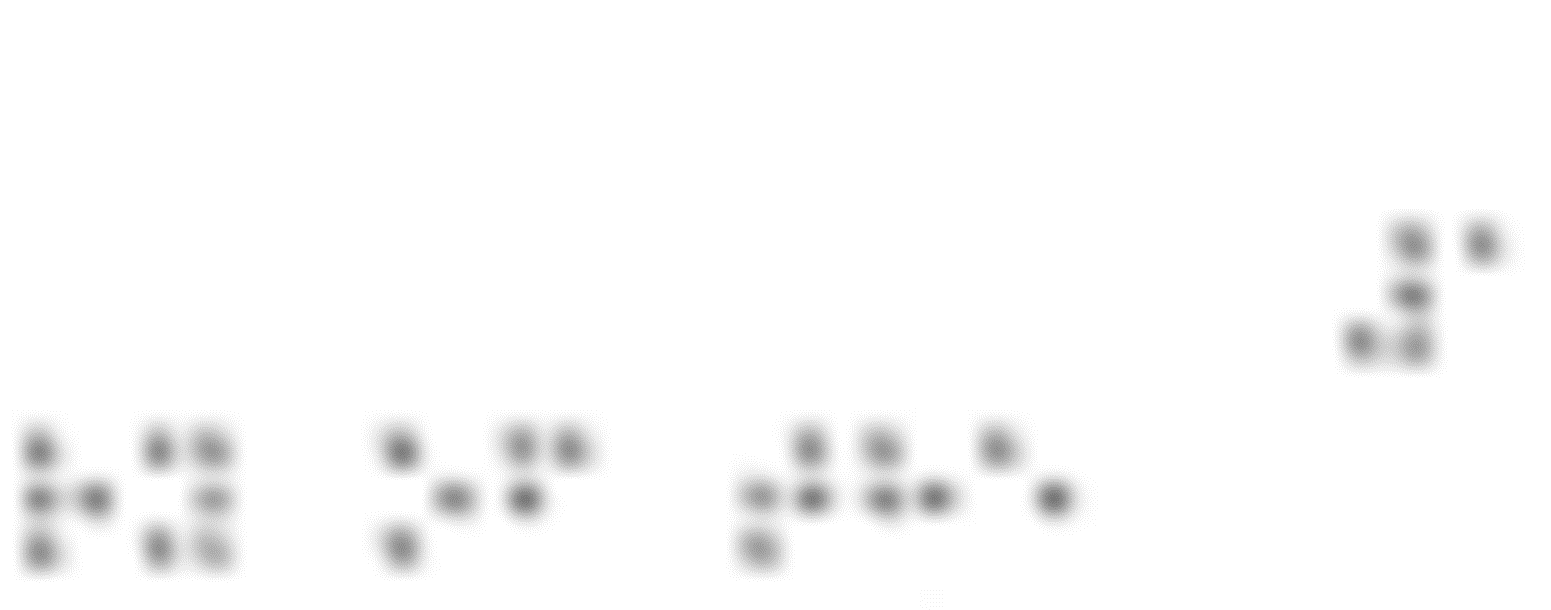
\includegraphics[width=.8\textwidth]{After medianBlur.png}
     \end{subfigure}
        \caption{zoomed look: Before and After applying the MedianBlur}
        \label{fig:Clear real braille samples}
\end{figure}\\
\quad in our case we only needed a small kernel of 3\textsuperscript{rd} degree
which has relatively low computational power.\\

\quad This concludes our preprocessing filters
section. We will now proceed to the next section, which focuses on
rotation correction.
\end{quote}\\

\newpage
\subsection{\textbf{Image Alignment and De-skewing } }\\
 The next challenge in preprocessing so then the image is ready for the detection step is De-skewing rotated images. This step is essential to enhance the accuracy of the next steps and to avoid over complicating the detection process.\\
\quad It is important to mention that the image must not be rotated with wide angles or else some of the dots will not scanned or partially scanned.\\
\quad To start facing the challenge we returned to the previous work by Isayed and Tahboub [4]. In their paper they have discussed many options to solve the skewing problem; linear regression method, standard deviation and Hough transform algorithm. We worked on both linear regression and Hough transform methods and found out that Hough transform method gives the most accurate results and the most generic for different examples and angles.\\
 \subsubsection{linear regression}
 \\
The idea in this method was to use the coordinates of the centers of the dot to find the angle of rotation. We used Hough circle transformation to find the coordinates, this is explained in chapter 5. We tried to find the angle using the linear equation Y=BX+A.
\begin{figure}[h!]
     \centering
        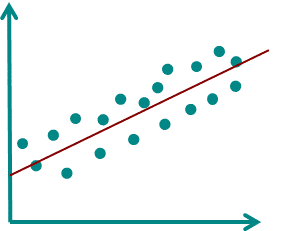
\includegraphics[width=0.3\textwidth]{Linear_regression_assumption_linearity.png}
        \caption{Scatter Plot with Linear Regression Line}
        \label{Scatter Plot with Linear Regression Line}
\end{figure}\\
 by calculating the slope of the straight line between two adjacent dots. The problem here is that the center detected by Hough circles method is not always the center of the dot. It might be shifted one or two pixels in any of the four directions. So, using only 2 adjacent dots is not effective.\\
 \quad We then started to work with 10 dots or more and try to find the best fitting line between the 10 dots and find the slope of this line.  for each 10 lines we find the slop and find the most repeated slope (mode of the slopes). from the slope we get the angle of rotation and use it to De-skew the image.
 The result of this method was not accurate having many problems:\\
 \begin{itemize}
    \item The slopes detected from each group of dots were not precise and gave different results.
    \item The angle chosen at the end was not accurate enough to continue to the next steps of the detection.
    \item This method was not generic for many Braille pages. It worked for one or two pages but then needed to be edited to be suitable for other pages.
\end{itemize}\\
\quad We tried to increase the number of dots in the group to find the best fitting line but that did not solve the problems we have. We also tried calculating the mean of the slopes instead of finding the mode but again all three problems were not solved. This pushed us to try other solutions.

\subsubsection{Hough line Transform method}
\\
The solution we tried next was to use the Hough transform to find the lines that connect the dots and find the angle of rotation. First we have to explain the how Hough transformation find the lines.\\

\textbf {Hough Line Transform}
\begin{enumerate}
    \item The Hough Line Transform is a transform used to detect straight lines.
    \item To apply the Transform, first an edge detection pre-processing is desirable.
\end{enumerate}\\

\textbf{How does it work?}

\begin{enumerate}
    \item A line in the image space can be expressed with two variables. For example:
    \begin{enumerate}
        \item In the Cartesian coordinate system: Parameters: (m, b).
        \item In the Polar coordinate system: Parameters: (r, $\theta$).
    \end{enumerate}
\end{enumerate}\\
\begin{figure}[h!]
     \centering
        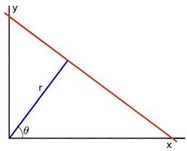
\includegraphics[width=0.6\textwidth]{Picture1.jpg}
        \caption{Representation of a Line in Cartesian and Polar Coordinate Systems}
        \label{Representation of a Line in Cartesian and Polar Coordinate Systems}
\end{figure}


For Hough Transforms, we will express lines in the Polar system. Hence, a line equation can be written as:\\
\[
y = \left(-\frac{\cos\theta}{\sin\theta}\right) x + \left(\frac{r}{\sin\theta}\right)
\]
Arranging the terms:
\[
r = x \cos\theta + y \sin\theta
\]

\begin{enumerate}
    \item In general, for each point \((x_0, y_0)\), we can define the family of lines that goes through that point as:
    \[
    r_\theta = x_0 \cdot \cos\theta + y_0 \cdot \sin\theta
    \]
    Meaning that each pair \((r_\theta, \theta)\) represents each line that passes by \((x_0, y_0)\).

    \clearpage
    \item If for a given \((x_0, y_0)\) we plot the family of lines that goes through it, we get a sinusoid. For instance, for \(x_0 = 8\) and \(y_0 = 6\) we get the following plot in figure  \ref{fig333} :

    \begin{figure}[h!]
     \centering
        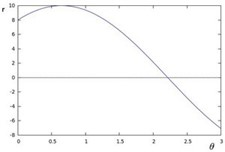
\includegraphics[width=0.6\textwidth]{Picture2.jpg}
        \caption{\(\theta - r\) plane for single selected point}
        \label{fig333}
    \end{figure}

    We consider only points such that \(r > 0\) and \(0 < \theta < 2\pi\).
    
    \item We can do the same operation above for all the points in an image. If the curves of two different points intersect in the plane \(\theta - r\), that means that both points belong to the same line. For instance, continuing with the example above and drawing the plot for two more points: \(x_1 = 4\), \(y_1 = 9\) and \(x_2 = 12\), \(y_2 = 3\), we get:
    \begin{figure}[h!]
     \centering
        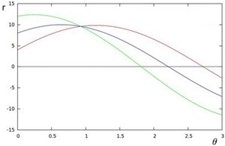
\includegraphics[width=0.6\textwidth]{Picture3.jpg}
        \caption{\(\theta - r\) plane for multiple selected point}
        \label{fig}
    \end{figure}
    The three plots intersect in one single point \((0.925, 9.6)\), these coordinates are the parameters \((\theta, r)\) of the line in which \((x_0, y_0)\), \((x_1, y_1)\), and \((x_2, y_2)\) lie.
    
    \item What does all the above mean? It means that, in general, a line can be detected by finding the number of intersections between curves. The more curves intersect, the more points lie on the line represented by that intersection. In general, we can define a threshold for the minimum number of intersections needed to detect a line.
    
    \item This is what the Hough Line Transform does. It keeps track of the intersections between curves of every point in the image. If the number of intersections is above some threshold, it declares it as a line with the parameters \((\theta, r_\theta)\) of the intersection point.
\end{enumerate}\\

\textbf{Standard and Probabilistic Hough Line Transform\\}

OpenCV implements two kinds of Hough Line Transforms:\\

\textbf{The Standard Hough Transform}
\begin{itemize}
    \item It consists of pretty much what we just explained in the previous section. It gives as a result a vector of pairs \((\theta, r_\theta)\).
    \item In OpenCV, it is implemented with the function \texttt{HoughLines()}.
\end{itemize}\\

\textbf{The Probabilistic Hough Line Transform}
\begin{itemize}
    \item A more efficient implementation of the Hough Line Transform. It gives as output the extremes of the detected lines \((x_0, y_0, x_1, y_1)\).
    \item In OpenCV, it is implemented with the function \texttt{HoughLinesP()}.
\end{itemize}

\subsubsection{Applying the Hough Transformation for Line Detection and page De-Skewing}
\quad To use the Hough transformation, we pass the scanned image through filtering process, discussed earlier in this chapter. The resulted black \& white image, shown previously in figure 4.13, is passed through edge detection filter that uses canny algorithm, which is going to be explained in details in chapter 5.  \\
\quad The next step is the Hough transformation. We used the OpenCV function HoughLinesP(). this function takes an input image and pass an array of lines as an output. The function also takes other parameters like minimum line length which was 90 pixels in our implementation and the maximum line gap, 200 pixels. These values were reached by trail to reach the best results.\\

\quad For illustration the lines are drawn on the input image to show the output of the function. Figure 4.19 compares between the input image and the output of the HoughLinesP() function. \\

The precision of the lines can be observed in Figure 4.19 (b). Most of the lines extracted are horizontal with a small angle to the x-axis. There are also some vertical lines with the same angle but to the y-axis. The diagonal lines are to be ignored as they are considered noise. \\

Some pages will have more vertical lines than horizontal lines so we rotate all the angles between 80 and 100 degrees with the horizontal axis by 90 degrees to add these lines to our next steps. We also removed any diagonal lines to avoid their effect while calculating the angle of rotation. We then calculate the mean of all the angles to find the angle of rotation. For example, the angle of rotation in figure 4.19 is -0.99469 degrees. \\



\begin{figure}[H]
\centering
\subfloat[rotated scanned image]{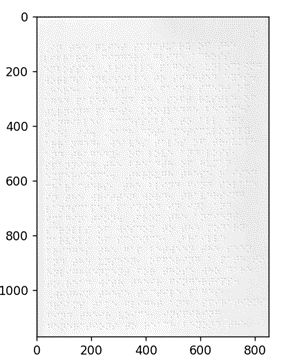
\includegraphics[width=0.6\linewidth]{Picture4.png}}\hfill
\subfloat[lines on the rotated page]{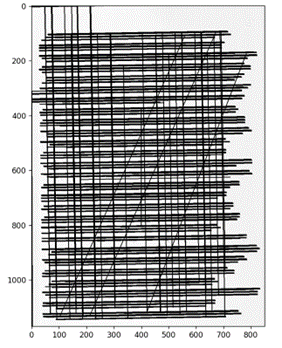
\includegraphics[width=0.6\linewidth]{Picture5.png}}\\
\caption{Using Hough line transform on rotated image}
\label{fig:num1235}
\end{figure}

\newpage


 The next step is to calculate the angle between the horizontal x-axis and the lines. That is easily done by finding two points of each line and calculate the slope as arctan the angle. \\



The angle of rotation is used to rotate the image using built in functions in python. The output of the rotation function is shown in figure 4.20. A border is added after rotation. We have chosen white border to blend with the background of the processed image. The additional border adds noise in the middle between the border and the image. This noise can be detected by the detection process coming next. So we have to remove that part even it is as small as in the figure. This is done by finely cropping the edges of the image to remove the noise without affecting any of the dots. The final image after cropping that can be used in the next steps of our project is shown in figure 4.20 (b). \\

\begin{figure}[h!]
     \centering
     \begin{subfigure}
         \centering
         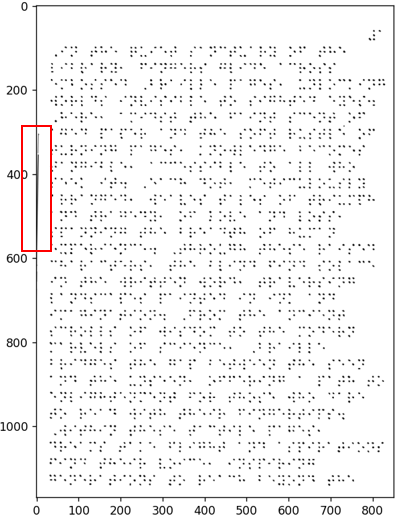
\includegraphics[width=.45\textwidth]{Picture6.png}
     \end{subfigure}
     \hfill
     \begin{subfigure}
         \centering
         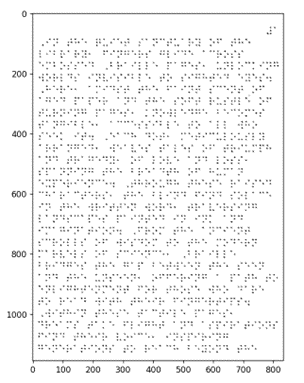
\includegraphics[width=.478\textwidth]{Picture7.png}
     \end{subfigure}
        \caption{(a) image after rotation \quad (b) image after cropping the edges }
        \label{fig:orientation}
\end{figure}
\textbf{\\ Discussion \\}
\\
\quad The rotation algorithm we used showed great results and the rotated images were almost the same accuracy as an upright scanned image. The system was tested with images rotated with angles between -2 and 2 degrees. the system was able to calculate the angle with accuracy to the fifth decimal point of a degree. \\
\quad One of the problems of rotated image is that the dots fades slightly compared to the upright image due to the kernel used in the filters. The tuning of the filters was done to be affective with all angles in the range we tested. However, the faded dots can affect the detection result but as our results show it does not exceed 1\% of the symbols and all these errors is detected and corrected by the correction part in our project.   \\